\documentclass[12pt]{article} \usepackage{jeep} \usepackage{unicode}
\usepackage{setspace} \usepackage[scaled]{helvet}
\renewcommand\familydefault{\sfdefault} \usepackage[T1]{fontenc}
\usepackage[numbers]{natbib} \usepackage{tabularx}
\usepackage[hidelinks]{hyperref} \hypersetup{ colorlinks, citecolor=black,
  filecolor=black, linkcolor=black, urlcolor=black } \usepackage{float}
\usepackage{graphicx} \usepackage{pdfpages} \usepackage{tabularx}
\newcommand\createfigure[2]{
  \begin{figure}[H]
    \centering \includegraphics[width=\textwidth]{#1}
    \caption{#2}
  \end{figure}}
\begin{document}
\linespread{1.0}
\begin{titlepage}
  \begin{center}
    \large{University of Puerto Rico\\
    Mayagüez Campus\\
    \vspace{\baselineskip}
    Department of Electrical and Computer Engineering\\}
    \vspace{6cm}
    \Huge{\underline{Insulin Temperature Warning System}\\}
    \vspace{0.5\baselineskip}
    \large by\\
    Fabio J. Matos Nieves\\
    Enrique Chompré\\
    Guillermo Colón\\
    Rubén Marrero\\
    \vspace{3.5cm}
    For: Professor Manuel Jimenez\\
    Course: INEL 4217 Seccion 096\\
    Date: Febuary 2, 2023\\
    \normalsize

  \end{center}
\end{titlepage}

\linespread{2.0}
\section{Hold a meeting with your project teammates and discuss your individual
  recommendations and provide a team agreed choice of:}
\subsection{Revised Top-level System View}
\createfigure{../Figures/global-system-view.png}{Top Level System View}
\subsection{Expected system life cycle with brief explanation of planned stages}
\begin{enumerate}
  \item Requirements Gathering: Entails discusing with a client the details for the particular problem at hand and defining a domain and solution scope.
  \item Conceptual Design: The high level overview of the proposed design for the client.
  \item Detailed Design: The low level, detailed plans for the design.
  \item Implementation: The actual purchasing of the necessary software and hardware, the prototyping and integration of all parts of the design.
  \item Testing: The verifying that all parts of the design function correctly in a verity of test cases.
  \item Deployment: The delivery and installation of the product to the customer.
\end{enumerate}
\subsection{System HW architecture (BDV2).}
\createfigure{../Figures/system-architecture-block-diagram.jpg}{System
  Architecture Block Diagram}
\newpage
\begin{center}
  \begin{tabularx}{\textwidth}{|X|X|}
    \hline
    Hardware (Sub-Unit) & Required processor resources (Sub-Unit)\\
    \hline
    Battery & VDD and GND pins on MCU\\
    \hline
    LED & 1 GPIO Pin\\
    \hline
    Bluetooth Module & TDX, RXD and 1 GPIO for enable (3 GPIO in total)\\
    \hline
    Temperature Sensor (Internal) & Increased power consumption\\
    \hline
    Total & 4 GPIO pins, VDD and GND pins and 1 internal temperature sensor\\
    \hline
  \end{tabularx}
\end{center}
\begin{center}
  \begin{tabularx}{\textwidth}{|X|X|}
    \hline
    Hardware (Main-Unit) & Required processor resources (Main-Unit)\\
    \hline
    Uninterruptible Power Supply & VDD and GND pins on MCU\\
    \hline
    Bluetooth Module & TDX, RXD and 1 GPIO for enable (3 GPIO in total)\\
    \hline
    Temperature Sensor (Internal) & Increased power consumption\\
    \hline
    Regulator & 1 GPIO Pin\\
    \hline
    Total & 4 GPIO pins, VDD and GND pins and 1 internal temperature sensor\\
    \hline
  \end{tabularx}
\end{center}
\subsection{Project Poster}
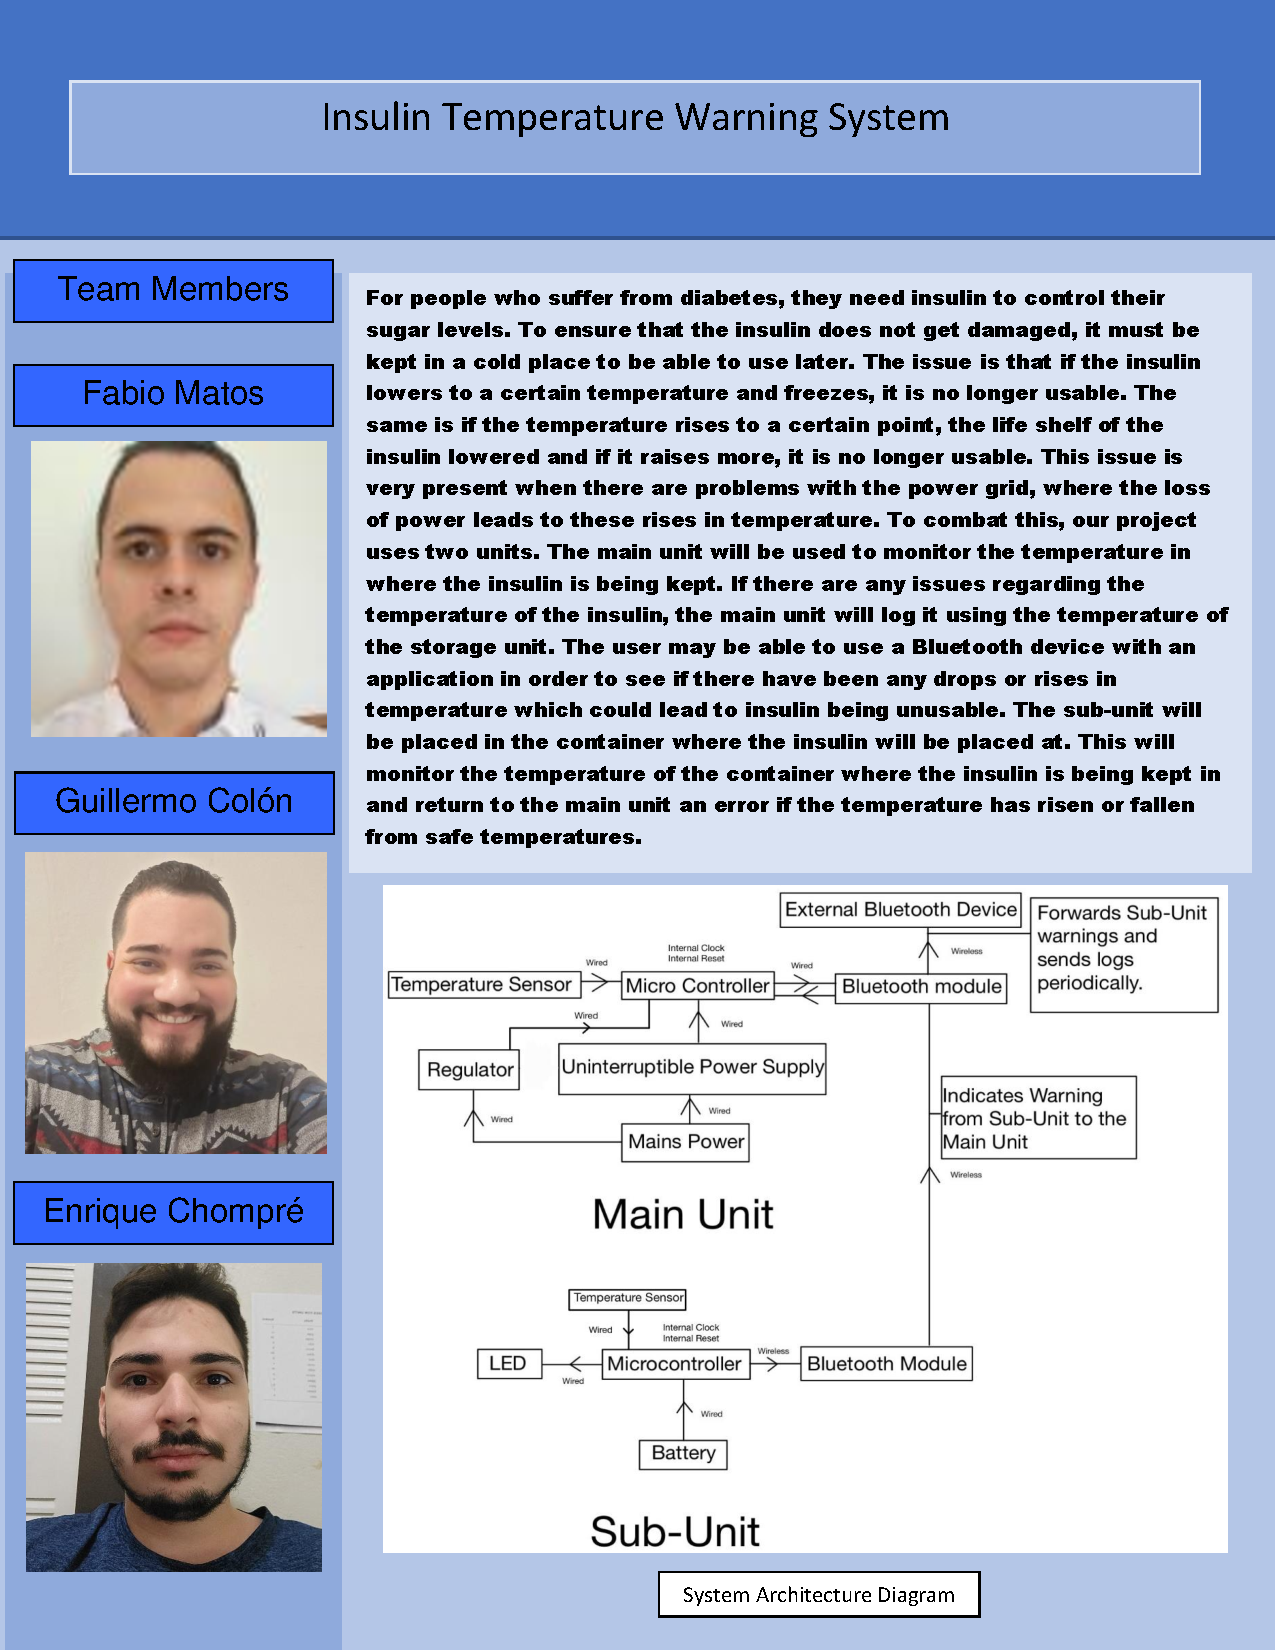
\includepdf[pages=-]{../Figures/project-poster.pdf}
\subsection{SW functionality B0.5}
\createfigure{../Figures/SW functionality B0.5.jpg}{Software Functionality}
\subsection{Processor selection}
\subsubsection{Provide a top-level description of the proposed functionality,
  and list the major software functions envisioned by this system.}
\begin{itemize}
  \item Sub-Unit: Checks the temperature of an individual box of insulin and if
        compliance is not met send an error to the main unit and lights and LED
        on the box.
        \begin{itemize}
          \item Hold the lot number and expiration date for the box of insulin.
          \item Check the current date and time.
          \item Check the current temperature of the box of insulin.
          \item Verify that the box of insulin meets safety standards.
          \item If compliance is not met, send an error top the main unit and
                light an LED on the insulin box.
        \end{itemize}
  \item Main-Unit:
        \begin{itemize}
          \item Check the current temperature.
          \item Check the current time.
          \item Check if mains power is available.
          \item Create a log file with the current temperature, power status and
                current time.
          \item Periodically send log file to a server.
          \item Forward warning signals from sub-units to a server and an
                applet.
          \item Forward temperature and power status warnings to a server and an
                applet.
        \end{itemize}
\end{itemize}
\subsubsection{List technical details of this design in terms of data type,
  speed requirements for real-time reactive operation, power source, size and
  weight, and two design constraints to be carried throughout the system
  design.}
In terms of data types the sub-units need to hold a 30 character lot number (240
bits in total), the current time (32 bits) and a 7 bit signed integer for the
temperature and an error code (4 bit integer). The main unit needs to hold the
current time (32 bits), power status (1 bit) and an array of lot numbers and
error codes $n\cdot244$ bits.\vspace{\baselineskip} \\
For the need of real-time operation, the sub-units are going to be asleep for the vast majority of the time (only waking up periodically to check the current status) and thus realtime operation is not needed. For the main unit, real time operation is not necessary but putting the unit to sleep is not viable since it waits for errors from sub-units.\vspace{\baselineskip}\\
In terms of size restrictions the main-unit is limited by the size of the UPS,
regulator and bluetooth module and since ideally it will be located in a place
where all the sub-units are within range, space and weight is not much of a
concern. However, for the subunits size and weight is a major concern since it
has to easily fit within a box of insulin and be easily attached to the box
without substantially increasing the weight of the boxes and thus shipping costs
for the manufacturers.\vspace{\baselineskip}\\
Where the main and subunits differ the most is in the power sources, the main unit uses a UPS and mains power for its daily operation and thus power efficiency is not much of a concern. In stark contrast, the sub-units only run on battery for at least two years, thus creating a power efficient design is critical for the sub-units.\\
The two main design constrains for both the main and sub units are cost and
environmental. In terms of cost both the main and sub-units need to be
inexpensive do be able to easily integrated into currently existing
manufacturing processes and storage facilities. In terms of the environment,
this design has to work in extended blackouts whilst still accurately reporting
data and verifying compliance.
\subsubsection{Based on your transient data type prediction, estimate the data
  memory requirements of this application. Briefly justify your estimate.}
In terms of data types the sub-units need to hold a 30 character lot number (240
bits in total), the current time (32 bits) and a 7 bit signed integer for the
temperature and an error code (4 bit integer) totaling 279 bits of RAM. The main
unit needs to hold the current time (32 bits), power status (1 bit), the current
temperature (7 bit signed integer) and an array of lot numbers and
error codes $n\cdot244$ bits totaling $40 + N\cdot244$ bits where N is the amount of error structures in memory. \vspace{\baselineskip}\\
\subsubsection{Processor selection. A table comparing the features of at least
  three processors.}
\begin{center}
  \begin{tabularx}{\textwidth}{|X|X|X|X|}
    \hline
    MCU & Dev Kit Availability & IDE Availability & Cost\\
    \hline
    MSP430FR2000 & Yes & Yes & \$0.276 per unit at 1ku\\
    \hline
    MSP430FR2100 & Yes & Yes & \$0.291 per unit at 1ku\\
    \hline
    MSP430FR2110 & Yes & Yes & \$0.305 per unit at 1ku\\
    \hline
  \end{tabularx}
  \begin{center}
    \begin{tabularx}{\textwidth}{|X|X|X|}
      \hline
      MCU & Advantages & Disadvantages\\
      \hline
      MSP430FR2000 & 12 GPIO pins, an RTC, 1 UART port and an integrated temperature sensor and is the cheapest out of the three options. & Having 1 UART port limits the amount of communication channels the MCU can use. \\
      \hline
      MSP430FR2100 & 12 GPIO pins, an RTC, 1 UART port and an integrated temperature sensor. & Having 1 UART port limits the amount of communication channels the MCU can use. \\
      \hline
      MSP430FR2110 & 12 GPIO pins, an RTC, 1 UART port and an integrated temperature sensor. & Having 1 UART port limits the amount of communication channels the MCU can use and is the most expensive out of the three options. \\
      \hline
    \end{tabularx}
  \end{center}
\end{center}
\subsubsection{Provide a recommendation of the processor to be used for this application.}
For the sub-units, at most, they need to hold the current time and 31 byte error data
structure in memory, thus the MSP430FR2000 would be an excellent choice for this
since they are the lowest cost MCU that meets the feature requirements. For the
main unit, the MSP430FR2110 would be great since it could potentially need to
hold and process donzens of error codes at a time, thus the extra ram would be
required for this case.
\section{A brief, 5-slide presentation of your approved project}
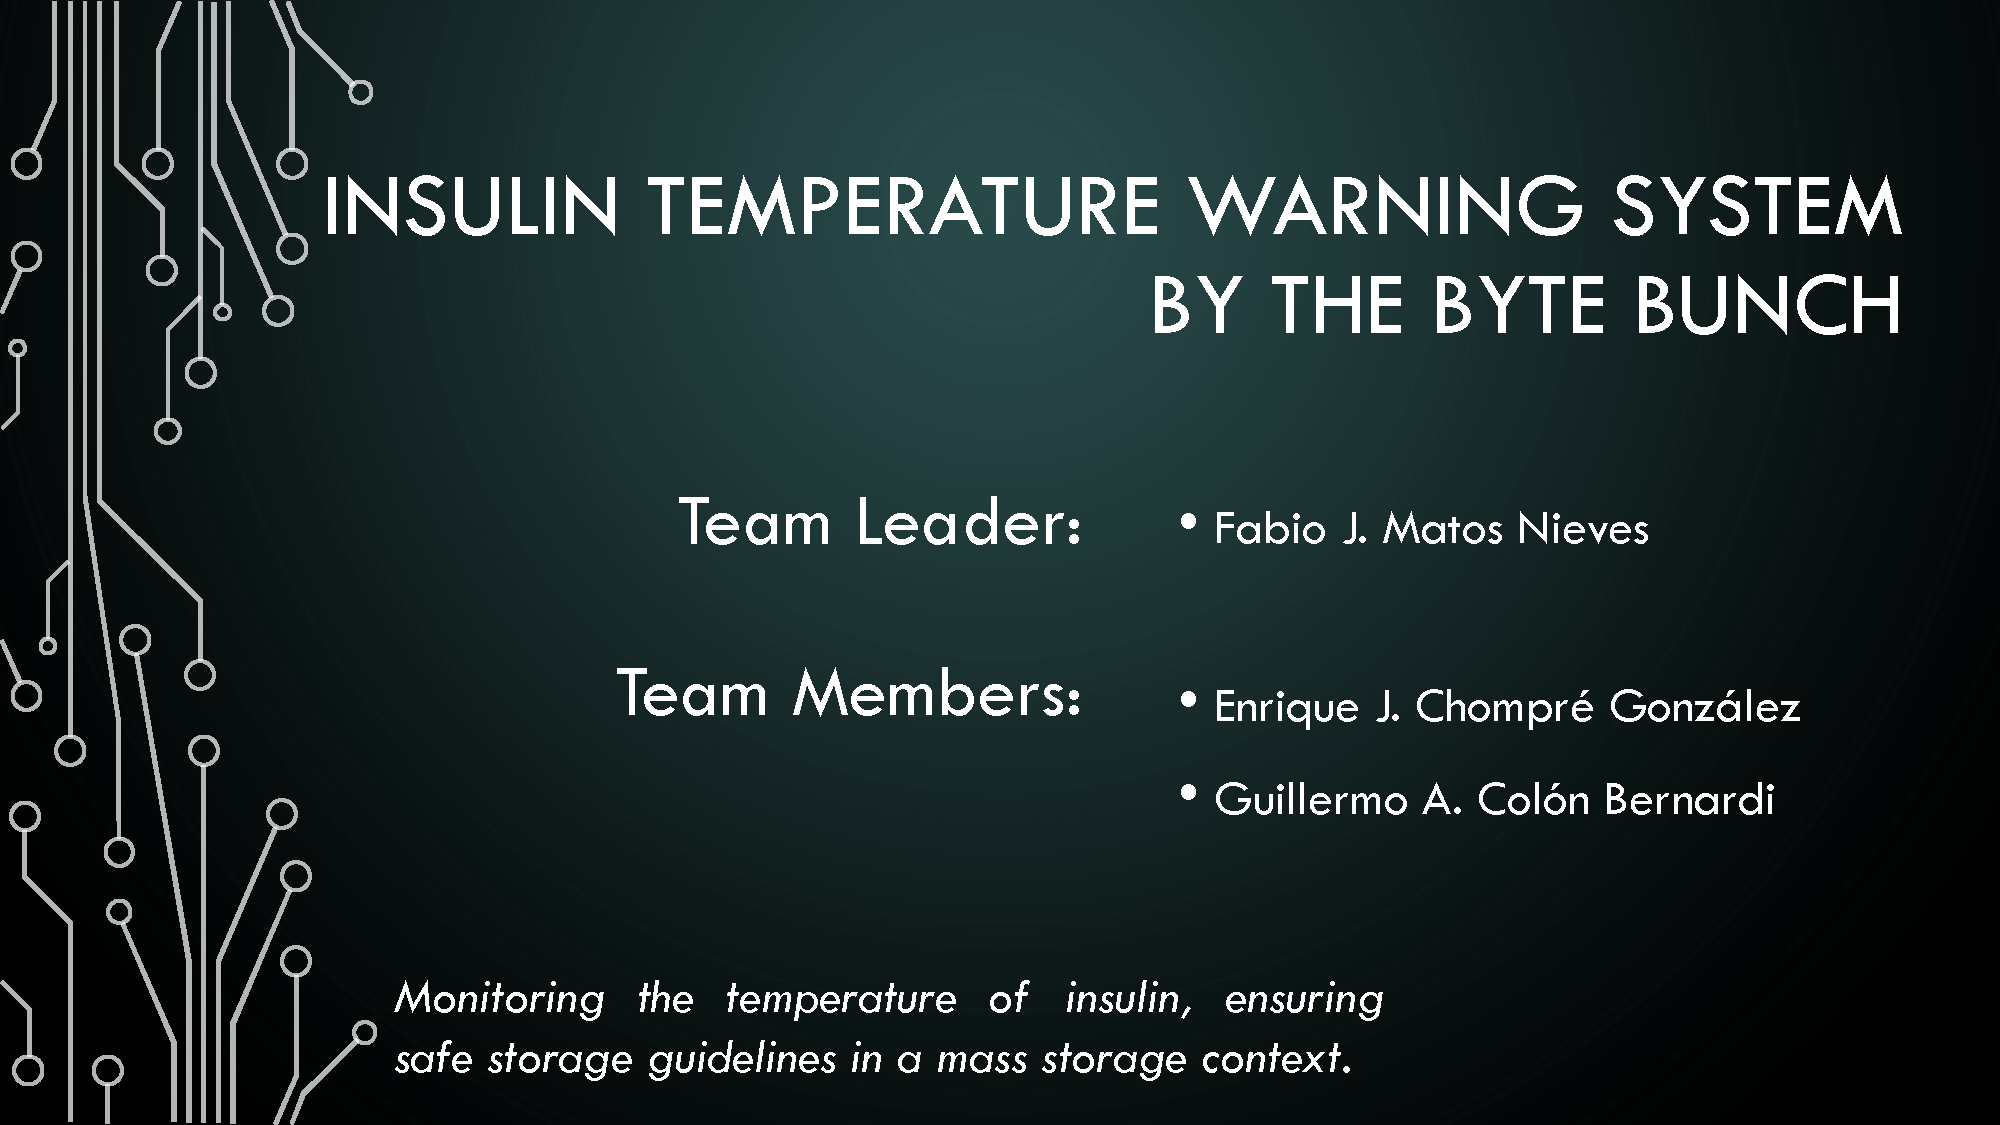
\includepdf[pages=-]{../Presentation/presentation.pdf}

\end{document}
